\documentclass[]{book}
\usepackage{lmodern}
\usepackage{amssymb,amsmath}
\usepackage{ifxetex,ifluatex}
\usepackage{fixltx2e} % provides \textsubscript
\ifnum 0\ifxetex 1\fi\ifluatex 1\fi=0 % if pdftex
  \usepackage[T1]{fontenc}
  \usepackage[utf8]{inputenc}
\else % if luatex or xelatex
  \ifxetex
    \usepackage{mathspec}
  \else
    \usepackage{fontspec}
  \fi
  \defaultfontfeatures{Ligatures=TeX,Scale=MatchLowercase}
\fi
% use upquote if available, for straight quotes in verbatim environments
\IfFileExists{upquote.sty}{\usepackage{upquote}}{}
% use microtype if available
\IfFileExists{microtype.sty}{%
\usepackage[]{microtype}
\UseMicrotypeSet[protrusion]{basicmath} % disable protrusion for tt fonts
}{}
\PassOptionsToPackage{hyphens}{url} % url is loaded by hyperref
\usepackage[unicode=true]{hyperref}
\hypersetup{
            pdftitle={The EMaC R Manual},
            pdfauthor={Alex Sciuto},
            pdfborder={0 0 0},
            breaklinks=true}
\urlstyle{same}  % don't use monospace font for urls
\usepackage{natbib}
\bibliographystyle{apalike}
\usepackage{color}
\usepackage{fancyvrb}
\newcommand{\VerbBar}{|}
\newcommand{\VERB}{\Verb[commandchars=\\\{\}]}
\DefineVerbatimEnvironment{Highlighting}{Verbatim}{commandchars=\\\{\}}
% Add ',fontsize=\small' for more characters per line
\usepackage{framed}
\definecolor{shadecolor}{RGB}{248,248,248}
\newenvironment{Shaded}{\begin{snugshade}}{\end{snugshade}}
\newcommand{\KeywordTok}[1]{\textcolor[rgb]{0.13,0.29,0.53}{\textbf{#1}}}
\newcommand{\DataTypeTok}[1]{\textcolor[rgb]{0.13,0.29,0.53}{#1}}
\newcommand{\DecValTok}[1]{\textcolor[rgb]{0.00,0.00,0.81}{#1}}
\newcommand{\BaseNTok}[1]{\textcolor[rgb]{0.00,0.00,0.81}{#1}}
\newcommand{\FloatTok}[1]{\textcolor[rgb]{0.00,0.00,0.81}{#1}}
\newcommand{\ConstantTok}[1]{\textcolor[rgb]{0.00,0.00,0.00}{#1}}
\newcommand{\CharTok}[1]{\textcolor[rgb]{0.31,0.60,0.02}{#1}}
\newcommand{\SpecialCharTok}[1]{\textcolor[rgb]{0.00,0.00,0.00}{#1}}
\newcommand{\StringTok}[1]{\textcolor[rgb]{0.31,0.60,0.02}{#1}}
\newcommand{\VerbatimStringTok}[1]{\textcolor[rgb]{0.31,0.60,0.02}{#1}}
\newcommand{\SpecialStringTok}[1]{\textcolor[rgb]{0.31,0.60,0.02}{#1}}
\newcommand{\ImportTok}[1]{#1}
\newcommand{\CommentTok}[1]{\textcolor[rgb]{0.56,0.35,0.01}{\textit{#1}}}
\newcommand{\DocumentationTok}[1]{\textcolor[rgb]{0.56,0.35,0.01}{\textbf{\textit{#1}}}}
\newcommand{\AnnotationTok}[1]{\textcolor[rgb]{0.56,0.35,0.01}{\textbf{\textit{#1}}}}
\newcommand{\CommentVarTok}[1]{\textcolor[rgb]{0.56,0.35,0.01}{\textbf{\textit{#1}}}}
\newcommand{\OtherTok}[1]{\textcolor[rgb]{0.56,0.35,0.01}{#1}}
\newcommand{\FunctionTok}[1]{\textcolor[rgb]{0.00,0.00,0.00}{#1}}
\newcommand{\VariableTok}[1]{\textcolor[rgb]{0.00,0.00,0.00}{#1}}
\newcommand{\ControlFlowTok}[1]{\textcolor[rgb]{0.13,0.29,0.53}{\textbf{#1}}}
\newcommand{\OperatorTok}[1]{\textcolor[rgb]{0.81,0.36,0.00}{\textbf{#1}}}
\newcommand{\BuiltInTok}[1]{#1}
\newcommand{\ExtensionTok}[1]{#1}
\newcommand{\PreprocessorTok}[1]{\textcolor[rgb]{0.56,0.35,0.01}{\textit{#1}}}
\newcommand{\AttributeTok}[1]{\textcolor[rgb]{0.77,0.63,0.00}{#1}}
\newcommand{\RegionMarkerTok}[1]{#1}
\newcommand{\InformationTok}[1]{\textcolor[rgb]{0.56,0.35,0.01}{\textbf{\textit{#1}}}}
\newcommand{\WarningTok}[1]{\textcolor[rgb]{0.56,0.35,0.01}{\textbf{\textit{#1}}}}
\newcommand{\AlertTok}[1]{\textcolor[rgb]{0.94,0.16,0.16}{#1}}
\newcommand{\ErrorTok}[1]{\textcolor[rgb]{0.64,0.00,0.00}{\textbf{#1}}}
\newcommand{\NormalTok}[1]{#1}
\usepackage{longtable,booktabs}
% Fix footnotes in tables (requires footnote package)
\IfFileExists{footnote.sty}{\usepackage{footnote}\makesavenoteenv{long table}}{}
\usepackage{graphicx,grffile}
\makeatletter
\def\maxwidth{\ifdim\Gin@nat@width>\linewidth\linewidth\else\Gin@nat@width\fi}
\def\maxheight{\ifdim\Gin@nat@height>\textheight\textheight\else\Gin@nat@height\fi}
\makeatother
% Scale images if necessary, so that they will not overflow the page
% margins by default, and it is still possible to overwrite the defaults
% using explicit options in \includegraphics[width, height, ...]{}
\setkeys{Gin}{width=\maxwidth,height=\maxheight,keepaspectratio}
\IfFileExists{parskip.sty}{%
\usepackage{parskip}
}{% else
\setlength{\parindent}{0pt}
\setlength{\parskip}{6pt plus 2pt minus 1pt}
}
\setlength{\emergencystretch}{3em}  % prevent overfull lines
\providecommand{\tightlist}{%
  \setlength{\itemsep}{0pt}\setlength{\parskip}{0pt}}
\setcounter{secnumdepth}{5}
% Redefines (sub)paragraphs to behave more like sections
\ifx\paragraph\undefined\else
\let\oldparagraph\paragraph
\renewcommand{\paragraph}[1]{\oldparagraph{#1}\mbox{}}
\fi
\ifx\subparagraph\undefined\else
\let\oldsubparagraph\subparagraph
\renewcommand{\subparagraph}[1]{\oldsubparagraph{#1}\mbox{}}
\fi

% set default figure placement to htbp
\makeatletter
\def\fps@figure{htbp}
\makeatother

\usepackage{booktabs}
\usepackage{amsthm}
\makeatletter
\def\thm@space@setup{%
  \thm@preskip=8pt plus 2pt minus 4pt
  \thm@postskip=\thm@preskip
}
\makeatother
\usepackage{booktabs}
\usepackage{longtable}
\usepackage{array}
\usepackage{multirow}
\usepackage{wrapfig}
\usepackage{float}
\usepackage{colortbl}
\usepackage{pdflscape}
\usepackage{tabu}
\usepackage{threeparttable}
\usepackage{threeparttablex}
\usepackage[normalem]{ulem}
\usepackage{makecell}
\usepackage{xcolor}

\title{The EMaC R Manual}
\author{Alex Sciuto}
\date{Last Updated Febuary 2020}

\begin{document}
\maketitle

{
\setcounter{tocdepth}{1}
\tableofcontents
}
\chapter{How to Install R}\label{download}

This is the EMaC manual for how to wrangle, analyze, and visualize data
in \textbf{R}. I will review a few key packages, in addition to explaing
their key functions, with real data examples.

There are two things you need to do to install R on your computer.
First, you would need to install the latest version of R which you would
download and install from this link:
\href{https://cloud.r-project.org/}{R-download}. Once you run and
install R onto your computer, you would need to install R-Studio. R
studio is the graphic user interface (GUI) where you can place all of
your R-code. Follow this link:
\href{https://rstudio.com/products/rstudio/download/}{R-Studio Desktop
Download}. Once you have these two programs installed, all you need to
do is launch R-studio Desktop and you are ready to go..

\chapter{Introduction to Programming in R}\label{intro}

Before you can do data wrangling, statiscs, and visualization using R
for cognitive psychology research, you need to learn the basic syntax in
R. This chapter will introduce the basics.

\section{Variables in R}\label{variables-in-r}

R can manipulate and wrangle all kinds of data, these data could be
stored in a handful of variables that we can then work with. The first
one we will be talking about is numeric.

\subsection{Numeric}\label{numeric}

a numeric is a number (including decimals) that can be stored within a
variable. Here is an example:

\textbf{\emph{\texttt{x\ =\ 2}}}

Here, we assigned the numeric value \texttt{2} to the variable
\texttt{x}. Thus, if we were to do arithemtic, \texttt{x} will be
treated as \texttt{2}. Moreover, there are specific functions in R we
can use in order to do arithmetic with numeric variables. Here are a few
examples:

\begin{longtable}[]{@{}ccc@{}}
\toprule
Arithemtic & R-Input & R-Output\tabularnewline
\midrule
\endhead
Addition: & \texttt{x\ +\ 2} & \texttt{4}\tabularnewline
Substraction: & \texttt{x\ -\ 2} & \texttt{0}\tabularnewline
Division: & \texttt{x\ /\ 2} & \texttt{1}\tabularnewline
Multiplication: & \texttt{x\ *\ 2} & \texttt{4}\tabularnewline
Exponent: & \texttt{x\ \^{}\ 2} & \texttt{4}\tabularnewline
\bottomrule
\end{longtable}

\subsection{Character}\label{character}

A character is a combination of characters (either letters and/or
numbers) that can be stored within a variable. Moreover, it is very
important that you place the character between quotation marks. Here is
an example:

\textbf{\emph{\texttt{x\ =\ "Cognitive\ Psychology"}}}

Here, we assigned the character value \texttt{"Cognitive\ Psychology"}
to the variable \texttt{x}. There are ways to manipulate character type
variables, and also modify them. However, we will touch on that later.

\subsection{Logical}\label{logical}

A logical can only have two possible values, \texttt{TRUE} and
\texttt{FALSE} that can be stored within a variable. This is not
typically a varaible type that you will need to assign variable values
to. However, the logical type variable is extremely important becuase a
lot of functions in R return a logical variable. We will dive into some
of these functions

\subsection{Vector}\label{vector}

A vector is multiple variables stored into one data-set. Vectors can
contain any variable type: character, numeric, string, and logical. When
you are declaring a a vector type variable, you typically have to use
the concatenate function \texttt{c()}. Here is an example:

\texttt{x\ =\ c(1,2,3,4)}

\texttt{x\ =\ c("I",\ "like",\ "Cognitive",\ "Psychology")}

\texttt{x\ =\ c(TRUE,\ FALSE,\ FALSE,\ TRUE)}

To reference a vector varaible, you need to use \texttt{{[}{]}} and
inside the brackets, you have to specify the index of where the given
variable in the vector is. Here is an example

\begin{Shaded}
\begin{Highlighting}[]
\NormalTok{x =}\StringTok{ }\KeywordTok{c}\NormalTok{(}\StringTok{"10"}\NormalTok{, }\StringTok{"20"}\NormalTok{, }\StringTok{"30"}\NormalTok{, }\StringTok{"40"}\NormalTok{)}
\NormalTok{x[}\DecValTok{4}\NormalTok{]}
\end{Highlighting}
\end{Shaded}

\begin{verbatim}
## [1] "40"
\end{verbatim}

Here, we assigned the numbers: \texttt{10,\ 20,\ 30,\ 40} to the vector
\texttt{x}. \texttt{"Cognitive\ Psychology"} to the variable \texttt{x}.
There are ways to manipulate character type variables, and also modify
them. However, we will touch on that later.

\section{Logical Operators}\label{logical-operators}

Now that you have a basic understanding of how variables work in R, the
next step is to learn how to use logical operators in order to specifiy
what are the specific conditions under which you want your variables to
be manipulated. The main way to do this in R is by using logical
operators.

\textbf{\emph{\texttt{x\ =\ 2}}}

Here, we assigned the numeric value \texttt{2} to the variable
\texttt{x}. Thus, if we were to apply logical operators to \texttt{x},
\texttt{x} will be treated as \texttt{2}. Here are examples of all of
the logical operators:

\begin{longtable}[]{@{}lccc@{}}
\toprule
Logical Operators & Description & R-Input & R-Output\tabularnewline
\midrule
\endhead
\textless{} & less than & x \textless{} 10 & TRUE\tabularnewline
\textless{}= & less than or equal to & x \textless{}= 2 &
TRUE\tabularnewline
\textgreater{} & greater than & x \textgreater{} 1 & TRUE\tabularnewline
\textgreater{}= & greater than or equal to & x \textgreater{}= 3 &
FALSE\tabularnewline
== & exactly equal to & x == 9 & FALSE\tabularnewline
!= & not equal to & x != 10 & FALSE\tabularnewline
!x & Not x & !x & FALSE\tabularnewline
x \textbar{}~y & x OR y & x == 10 \textbar{}~x != 10 &
TRUE\tabularnewline
x \& y & x AND y & x == 10 \&x != 10 & FALSE\tabularnewline
\bottomrule
\end{longtable}

\chapter{Introduction to Data
Wrangling}\label{introduction-to-data-wrangling}

To introduce data wrangling, we will be working with a dataset from a
study conducted in our lab. Here are the details of the study in order
to understand the data manipulation more:

\section{The study}\label{the-study}

On each trial in this experiment (n = 174), each participant (n = 84)
sees a target word very briefly (e.g., word) and then is prompted to
select which of two letters was in a particular position of that word
(e.g., \_ \_ \_ ↓) - one letter was in the presented word (e.g., D) and
the other letter is in an orthographic neighbor of the word (e.g., K).
This is a 2 (visual field) x 3 (sentence context) experimental design:
the target word is either presented in the fovea (i.e., center of the
screen) or the parafovea (i.e., 3 degrees to the right of fixation).
Prior to the target word, they see a sentence context presented via
Rapid Serial Visual Presentation (RSVP) that constrains to target (i.e.,
makes the presented word predictable and the orthographic neighbor
implausible), constrains to the alternative (i.e., makes the
orthographic neighbor predictable and the presented word implausible),
or is neutral (i.e., makes neither word predictable but both of them
plausible). In addition, we collect data about the individual subjects'
language ability (i.e., their z-score on some test relative to the other
participants), including spelling recognition (i.e., circle which words
are spelled wrong), spelling dictation (i.e., write out words that they
hear said), and phonological decoding (i.e., read aloud a list of words
and a list of nonwords), and information about the lexical properties of
the words (e.g., word frequency, cloze probability, orthographic
neighborhood size, phonological neighborhood size, clustering
coefficient, orthographic similarity to other words, which of the two
words is higher frequency).

\section{Loading in Data}\label{loading-in-data}

\subsection{Loading Packages}\label{loading-packages}

Before we start wrangling the data, we need to load in the packages we
are using. In this lab, most of the data wrangling tools we will be
using will be located in the \texttt{tidyverse()} package. What is a
package? It is simply a group of functions that group of developers made
that makes computations easier. To learn more about the
\texttt{tidyverse} package, you may click on this
\href{https://www.tidyverse.org/}{link} and read on it! For the data
wrangling we will be doing in this section, we will be primarily using a
package within tidyverse called \texttt{dplyr}. to load in the package,
simply type in the following code. What this code is saying is IF you
don't have the \texttt{tidyverse} installed, THEN install the package.
After that, load the \texttt{tidyverse} with the \texttt{library()}
function.

\begin{Shaded}
\begin{Highlighting}[]
\ControlFlowTok{if}\NormalTok{(}\OperatorTok{!}\KeywordTok{require}\NormalTok{(tidyverse))\{}
    \KeywordTok{install.packages}\NormalTok{(}\StringTok{"tidyverse"}\NormalTok{)}
\NormalTok{\}}
\KeywordTok{library}\NormalTok{(tidyverse) }
\end{Highlighting}
\end{Shaded}

\subsection{setting the working
directory}\label{setting-the-working-directory}

Now that we have the packages that we need, we need to load up our
directory. What is a directory? It is essentially the folder we will be
using to read in files, or export files into. In this directory, we have
our data set of interest, \texttt{Topgown\_Data}

\subsection{Reading in Data}\label{reading-in-data}

Now that we have our working directory set we can use the
\texttt{read\_csv()} function which requires one minimum argument to
work which is the name of your \texttt{.csv} file. Here we are setting
the variable \texttt{mydata} to the contents within the \texttt{.csv}
file. It stores the contents of \texttt{Topgown\_Data.csv} in what is
called a data frame. What is a dataframe? it is simply a matrix where
each row constitutes a variable (which can be any type you want), and
rows are observations.

\begin{Shaded}
\begin{Highlighting}[]
\NormalTok{mydata =}\StringTok{ }\KeywordTok{read_csv}\NormalTok{(}\StringTok{"TopGown_Data.csv"}\NormalTok{, }\DataTypeTok{skip_empty_rows =} \OtherTok{TRUE}\NormalTok{)}
\end{Highlighting}
\end{Shaded}

X1

Participants

visual\_field

constrained\_to

presented\_word

predicted\_word

question

correct\_answer

item\_pair

Items

probe\_position

RT

accuracy

zTOWRE\_Word

zTOWRE\_Nonword

zSpelling\_Dictation

zSpelling\_Recogntion

zAll

zSpell

zTOWRE

OrthoN\_T

OrthoCC\_T

PhonoN\_T

Freq\_T

Freq\_P

OrthoCC\_P

OLD

Higher\_Freq

1

tg011

Fovea

A

cage

cape

NA

NA

19

37

3

2986.73

1

-1.749307

0.071771

-0.0918699

1.155124

-0.1535705

0.531627

-0.838768

13

0.0000001

17

9.048

8.605

0.0000000

1.10

Target

2

tg011

Parafovea

N

ache

acne

Were they very frustrated?

Y

83

165

3

4146.67

1

-1.749307

0.071771

-0.0918699

1.155124

-0.1535705

0.531627

-0.838768

3

1.5000000

23

6.741

6.284

1.5000000

1.75

Target

3

tg011

Fovea

A

male

sale

NA

NA

37

73

1

2496.54

1

-1.749307

0.071771

-0.0918699

1.155124

-0.1535705

0.531627

-0.838768

27

0.0000000

59

10.978

11.466

0.0000000

1.00

Alternative

4

tg011

Fovea

A

leaf

loaf

NA

NA

70

139

2

1845.46

1

-1.749307

0.071771

-0.0918699

1.155124

-0.1535705

0.531627

-0.838768

9

0.0500000

29

8.861

7.109

0.5000000

1.75

Target

5

tg011

Parafovea

T

step

stop

NA

NA

7

14

3

2125.17

1

-1.749307

0.071771

-0.0918699

1.155124

-0.1535705

0.531627

-0.838768

7

0.1666667

11

10.691

11.478

0.0416667

1.50

Alternative

6

tg011

Fovea

N

mint

mind

NA

NA

24

48

4

1415.47

1

-1.749307

0.071771

-0.0918699

1.155124

-0.1535705

0.531627

-0.838768

16

0.0000005

17

11.344

11.784

0.0000001

1.25

Alternative

7

tg011

Parafovea

A

cast

case

NA

NA

20

40

4

3168.45

1

-1.749307

0.071771

-0.0918699

1.155124

-0.1535705

0.531627

-0.838768

19

0.0000000

28

10.102

12.204

0.0000000

1.00

Alternative

8

tg011

Fovea

A

golf

wolf

NA

NA

76

151

1

3765.47

1

-1.749307

0.071771

-0.0918699

1.155124

-0.1535705

0.531627

-0.838768

4

0.0000000

2

9.254

9.979

0.0000000

1.90

Alternative

9

tg011

Fovea

N

mane

maze

NA

NA

3

6

3

1503.80

1

-1.749307

0.071771

-0.0918699

1.155124

-0.1535705

0.531627

-0.838768

27

0.0000000

59

6.238

8.775

0.0000001

1.25

Alternative

10

tg011

Parafovea

N

name

fame

NA

NA

17

33

1

1565.79

1

-1.749307

0.071771

-0.0918699

1.155124

-0.1535705

0.531627

-0.838768

11

0.0041667

21

12.604

8.714

0.0000000

1.15

Target

\section{Dplyr() Package}\label{dplyr-package}

We will now be wrangling this new dataset we imported into R using
several \texttt{dplyr} functions. These are the ones we will be
covering. In the following sections I will explain what each functions
does in detial.

\begin{longtable}[]{@{}cl@{}}
\toprule
\begin{minipage}[b]{0.21\columnwidth}\centering\strut
Function\strut
\end{minipage} & \begin{minipage}[b]{0.18\columnwidth}\raggedright\strut
Description\strut
\end{minipage}\tabularnewline
\midrule
\endhead
\begin{minipage}[t]{0.21\columnwidth}\centering\strut
select()\strut
\end{minipage} & \begin{minipage}[t]{0.18\columnwidth}\raggedright\strut
keeps only the variables you mention\strut
\end{minipage}\tabularnewline
\begin{minipage}[t]{0.21\columnwidth}\centering\strut
summarize()\strut
\end{minipage} & \begin{minipage}[t]{0.18\columnwidth}\raggedright\strut
Create new variables summarizing the variables of an existing
table\strut
\end{minipage}\tabularnewline
\begin{minipage}[t]{0.21\columnwidth}\centering\strut
group\_by()\strut
\end{minipage} & \begin{minipage}[t]{0.18\columnwidth}\raggedright\strut
takes an existing table and converts it into a grouped table where
operations are performed ``by group''\strut
\end{minipage}\tabularnewline
\begin{minipage}[t]{0.21\columnwidth}\centering\strut
arrange()\strut
\end{minipage} & \begin{minipage}[t]{0.18\columnwidth}\raggedright\strut
Order table rows by an expression involving its variables\strut
\end{minipage}\tabularnewline
\begin{minipage}[t]{0.21\columnwidth}\centering\strut
filter()\strut
\end{minipage} & \begin{minipage}[t]{0.18\columnwidth}\raggedright\strut
choose rows/cases where conditions are true.\strut
\end{minipage}\tabularnewline
\begin{minipage}[t]{0.21\columnwidth}\centering\strut
mutate()\strut
\end{minipage} & \begin{minipage}[t]{0.18\columnwidth}\raggedright\strut
adds new variables and preserves existing ones\strut
\end{minipage}\tabularnewline
\bottomrule
\end{longtable}

\subsection{select()}\label{select}

For this particular experiment we have two independent variables of
interest: \texttt{visual\_field} and \texttt{constrained\_to}; and four
participant variables of interest:
\texttt{zTOWRE\_Word},\texttt{zTOWRE\_Nonword},
\texttt{zSpelling\_Dictation},\texttt{zSpelling\_Recogntion}. What if we
are only interested in these variables, and we don't particularly need
word level variables such as \texttt{ortho\_N}, or \texttt{phono\_N}. We
can then select these variables.

For this particular function, the first argument is going to be the
dataset of interest. the dataset for we will be selecting from is
\texttt{mydata}. The following arguments are simply the columns you
would like to keep.

\begin{Shaded}
\begin{Highlighting}[]
\NormalTok{dplyr}\OperatorTok{::}\KeywordTok{select}\NormalTok{(mydata, Participants, visual_field, constrained_to, zTOWRE_Word,zTOWRE_Nonword,   zSpelling_Dictation,zSpelling_Recogntion)}
\end{Highlighting}
\end{Shaded}

Participants

visual\_field

constrained\_to

zTOWRE\_Word

zTOWRE\_Nonword

zSpelling\_Dictation

zSpelling\_Recogntion

tg011

Fovea

A

-1.749307

0.071771

-0.0918699

1.155124

tg011

Parafovea

N

-1.749307

0.071771

-0.0918699

1.155124

tg011

Fovea

A

-1.749307

0.071771

-0.0918699

1.155124

tg011

Fovea

A

-1.749307

0.071771

-0.0918699

1.155124

tg011

Parafovea

T

-1.749307

0.071771

-0.0918699

1.155124

tg011

Fovea

N

-1.749307

0.071771

-0.0918699

1.155124

tg011

Parafovea

A

-1.749307

0.071771

-0.0918699

1.155124

tg011

Fovea

A

-1.749307

0.071771

-0.0918699

1.155124

tg011

Fovea

N

-1.749307

0.071771

-0.0918699

1.155124

tg011

Parafovea

N

-1.749307

0.071771

-0.0918699

1.155124

\subsubsection{The Pipe (\%\textgreater{}*\%)}\label{the-pipe}

However, another way I would suggest writing code like this is to use a
function in the \texttt{tidyverse} called the pipe
(\texttt{\%\textgreater{}\%}). Like the \texttt{select()} function, the
first argument in all \texttt{tidyverse} functions will be your dataset
of interest. The pipe simply gets a dataset, and pushes it into the
first argument of a function. Here is an example.

\begin{Shaded}
\begin{Highlighting}[]
\NormalTok{mydata }\OperatorTok\StringTok{ }\NormalTok{dplyr}\OperatorTok{::}\KeywordTok{select}\NormalTok{(Participants, visual_field, constrained_to, zTOWRE_Word,zTOWRE_Nonword,    zSpelling_Dictation,zSpelling_Recogntion) }\OperatorTok
\StringTok{  }\NormalTok{dplyr}\OperatorTok{::}\KeywordTok{select}\NormalTok{(Participants, visual_field, constrained_to)}
\end{Highlighting}
\end{Shaded}

Participants

visual\_field

constrained\_to

tg011

Fovea

A

tg011

Parafovea

N

tg011

Fovea

A

tg011

Fovea

A

tg011

Parafovea

T

tg011

Fovea

N

tg011

Parafovea

A

tg011

Fovea

A

tg011

Fovea

N

tg011

Parafovea

N

In this regard, the pipe follows simple logic. Once a dataset is
manipulated by one function, you pass it to the next function.

\subsection{group\_by() \& summarise()}\label{group_by-summarise}

However, let us say we are particularly interested in the values of one
variable. For example, word properties. Therefore, we would need to
compile a new dataset that summarizes word properties, such as
orthographic neighborhood size. So in this example we will create a
dataframe summarized by the presented word.

\begin{Shaded}
\begin{Highlighting}[]
\NormalTok{mydata }\OperatorTok\StringTok{ }\NormalTok{dplyr}\OperatorTok{::}\KeywordTok{select}\NormalTok{(Participants, visual_field, constrained_to, presented_word, OrthoN_T) }\OperatorTok
\StringTok{  }\KeywordTok{group_by}\NormalTok{(presented_word) }\OperatorTok
\StringTok{  }\NormalTok{dplyr}\OperatorTok{::}\KeywordTok{summarise}\NormalTok{(}\DataTypeTok{OrthoN_T =} \KeywordTok{mean}\NormalTok{(OrthoN_T))}
\end{Highlighting}
\end{Shaded}

presented\_word

OrthoN\_T

ache

3

acne

4

ants

7

arts

8

aunt

6

ball

20

bats

23

beef

6

bees

20

bell

15

\subsection{arrange()}\label{arrange}

Let us say that we are still interested in neighborhood size of a
particular target word. we can arrange the these variables so we can
display the the words from lowest orthographic neighborhood size to
higher orthographic neighborhood size. For this we can use the arrange
function, which sorts a particular variable of interest in ascending or
descending order.

\begin{Shaded}
\begin{Highlighting}[]
\NormalTok{mydata }\OperatorTok\StringTok{ }\NormalTok{dplyr}\OperatorTok{::}\KeywordTok{select}\NormalTok{(Participants, visual_field, constrained_to, presented_word, OrthoN_T, Freq_T) }\OperatorTok
\StringTok{  }\KeywordTok{group_by}\NormalTok{(presented_word) }\OperatorTok
\StringTok{  }\NormalTok{dplyr}\OperatorTok{::}\KeywordTok{summarise}\NormalTok{(}\DataTypeTok{OrthoN_T =} \KeywordTok{mean}\NormalTok{(OrthoN_T)) }\OperatorTok
\StringTok{  }\NormalTok{dplyr}\OperatorTok{::}\KeywordTok{arrange}\NormalTok{(OrthoN_T)}
\end{Highlighting}
\end{Shaded}

presented\_word

OrthoN\_T

ache

3

film

3

gyms

3

wolf

3

womb

3

acne

4

clue

4

debt

4

drum

4

golf

4

\subsection{filter()}\label{filter}

Let us say that not only are we interested in orthographic neigbhorhood
size, but we want to know orthographic neighborhood size for a
particular condition in our study. We can then use the \texttt{filter()}
function, and only keep the trails that are within the condition of
interest. For this example, we are interested when the sentence is
constraining toward the target word and when the target word is
presented in the parafovea.

\begin{Shaded}
\begin{Highlighting}[]
\NormalTok{mydata }\OperatorTok\StringTok{ }\NormalTok{dplyr}\OperatorTok{::}\KeywordTok{select}\NormalTok{(Participants, visual_field, constrained_to, presented_word, OrthoN_T, Freq_T) }\OperatorTok
\StringTok{  }\KeywordTok{filter}\NormalTok{(visual_field }\OperatorTok{==}\StringTok{ "Parafovea"} \OperatorTok{&}\StringTok{ }\NormalTok{constrained_to }\OperatorTok{==}\StringTok{ "T"}\NormalTok{) }\OperatorTok
\StringTok{  }\KeywordTok{group_by}\NormalTok{(presented_word, visual_field, constrained_to) }\OperatorTok
\StringTok{  }\NormalTok{dplyr}\OperatorTok{::}\KeywordTok{summarise}\NormalTok{(}\DataTypeTok{OrthoN_T =} \KeywordTok{mean}\NormalTok{(OrthoN_T)) }\OperatorTok
\StringTok{  }\NormalTok{dplyr}\OperatorTok{::}\KeywordTok{arrange}\NormalTok{(OrthoN_T)}
\end{Highlighting}
\end{Shaded}

presented\_word

visual\_field

constrained\_to

OrthoN\_T

ache

Parafovea

T

3

film

Parafovea

T

3

gyms

Parafovea

T

3

wolf

Parafovea

T

3

womb

Parafovea

T

3

acne

Parafovea

T

4

clue

Parafovea

T

4

debt

Parafovea

T

4

drum

Parafovea

T

4

golf

Parafovea

T

4

\subsection{mutate()}\label{mutate}

Let us say that we are not only interested in word properties like
orthographic neighborhood size, but also the spelling ability of
particular participants. In this study we have four spelling tests,
which were measured through the following variables:
\texttt{zTowre\_Word}, \texttt{zTowre\_Nonword},
\texttt{Spelling\_Dictation}, \texttt{Spelling\_Recogntion}. However,
these are a lot of measures. what if we wanted to know the average
between all of these measures for each participant? we can use the
mutate function to do this.

\begin{Shaded}
\begin{Highlighting}[]
\NormalTok{mydata }\OperatorTok\StringTok{ }\NormalTok{dplyr}\OperatorTok{::}\KeywordTok{select}\NormalTok{(Participants, zTOWRE_Word, zTOWRE_Nonword, zSpelling_Dictation, zSpelling_Recogntion) }\OperatorTok
\StringTok{  }\KeywordTok{group_by}\NormalTok{(Participants) }\OperatorTok
\StringTok{  }\NormalTok{dplyr}\OperatorTok{::}\KeywordTok{summarise}\NormalTok{(}\DataTypeTok{zTOWRE_Word =} \KeywordTok{mean}\NormalTok{(zTOWRE_Word), }
                   \DataTypeTok{zTOWRE_Nonword =} \KeywordTok{mean}\NormalTok{(zTOWRE_Nonword), }
                   \DataTypeTok{zSpelling_Dictation =} \KeywordTok{mean}\NormalTok{(zSpelling_Dictation), }
                   \DataTypeTok{zSpelling_Recogntion =} \KeywordTok{mean}\NormalTok{(zSpelling_Recogntion)) }\OperatorTok
\StringTok{  }\NormalTok{dplyr}\OperatorTok{::}\KeywordTok{mutate}\NormalTok{(}\DataTypeTok{aggregated_spelling =}\NormalTok{ ((zTOWRE_Word }\OperatorTok{+}\StringTok{ }\NormalTok{zTOWRE_Nonword }\OperatorTok{+}\StringTok{ }\NormalTok{zSpelling_Dictation }\OperatorTok{+}\StringTok{ }\NormalTok{zSpelling_Recogntion)}\OperatorTok{/}\DecValTok{4}\NormalTok{))}
\end{Highlighting}
\end{Shaded}

Participants

zTOWRE\_Word

zTOWRE\_Nonword

zSpelling\_Dictation

zSpelling\_Recogntion

aggregated\_spelling

derp033

1.6354380

0.7156786

0.8383130

1.3936520

1.1457704

derp044

-0.6333223

0.5317050

-0.0918699

-0.7923070

-0.2464486

derp055

0.2251274

0.6236918

-0.7895071

0.2705651

0.0824693

derp066

-1.1483920

-1.1240570

-2.8824190

-1.4607150

-1.6538958

derp071

-0.3757874

-0.1122026

0.6057672

0.6449458

0.1906808

\chapter{Plotting}\label{plotting}

Now that we have a basic understanding of how to wrangle data, now we
want to graphically explain the data we are wrangling. For this chapter
we will be using \texttt{ggplot} package to further understand the data.
However, before we go into plotting specific things about the data, we
need to learn the grammar of plotting with \texttt{ggplot} in general

\section{ggplot grammar}\label{ggplot-grammar}

You can think of the grammar of graphics as a systematic approach for
describing the components of a graph. It has seven components (the ones
in bold are required to be specifed explicitly in ggplot2):

\begin{itemize}
\tightlist
\item
  \textbf{\emph{Data}}

  \begin{itemize}
  \tightlist
  \item
    data that you're feeding into a plot.
  \end{itemize}
\item
  \textbf{\emph{Aesthetic mappings}}

  \begin{itemize}
  \tightlist
  \item
    How are variables (columns) from your data connect to a visual
    dimension? Horizontal positioning, vertical positioning, size,
    colour, shape, etc. These visual dimensions are called
    ``aesthetics''
  \end{itemize}
\item
  \textbf{\emph{Geometric objects}}

  \begin{itemize}
  \tightlist
  \item
    What are the objects that are actually drawn on the plot? A point, a
    line, a bar, a histogram, a density, etc.
  \end{itemize}
\item
  Scales

  \begin{itemize}
  \tightlist
  \item
    How is a variable mapped to its aesthetic? Will it be mapped
    linearly? On a log scale? Something else? This includes things like
    the color scale e.g., c(control, treatment\_1, treatment\_2)
    -\textgreater{} c(``blue'', ``green'', ``red'')
  \end{itemize}
\item
  Statistical transformations

  \begin{itemize}
  \tightlist
  \item
    Whether and how the data are combined/transformed before being
    plotted e.g., in a bar chart, data are transformed into their
    frequencies; in a box-plot, data are transformed to a five-number
    summary.
  \end{itemize}
\item
  Coordinate system

  \begin{itemize}
  \tightlist
  \item
    This is a specification of how the position aesthetics (x and y) are
    depicted on the plot. For example, rectangular/cartesian, or polar
    coordinates.
  \end{itemize}
\item
  Facet

  \begin{itemize}
  \tightlist
  \item
    This is a specification of data variables that partition the data
    into smaller ``sub plots'', or panels. These components are like
    parameters of statistical graphics, defining the ``space'' of
    statistical graphics. In theory, there is a one-to-one mapping
    between a plot and its grammar components, making this a useful way
    to specify graphics.
  \end{itemize}
\end{itemize}

\subsection{Example: Scatterplot
Grammar}\label{example-scatterplot-grammar}

Let us say that we are interested in how specific word properties relate
to one another, and how correlated they are. With this information we
can learn specific detials about the nature of our linguistic stimuli,
which is very important in psycholinguistics. So for this example we are
going to plot the orthographic neighborhood size of the target word and
word frequency.

\begin{Shaded}
\begin{Highlighting}[]
\NormalTok{mydata }\OperatorTok\StringTok{ }\KeywordTok{ggplot}\NormalTok{(}\KeywordTok{aes}\NormalTok{(}\DataTypeTok{x =}\NormalTok{ OrthoN_T, }\DataTypeTok{y =}\NormalTok{ Freq_T)) }\OperatorTok{+}\StringTok{ }\CommentTok{# this defines the x and y axes of the plot}
\StringTok{  }\KeywordTok{geom_point}\NormalTok{() }\OperatorTok{+}\StringTok{ }\CommentTok{# this adds geometric objects}
\StringTok{  }\KeywordTok{theme_update}\NormalTok{(}\DataTypeTok{plot.title =} \KeywordTok{element_text}\NormalTok{(}\DataTypeTok{hjust =} \FloatTok{0.5}\NormalTok{)) }\OperatorTok{+}\StringTok{ }\CommentTok{# this line centers the title}
\StringTok{  }\KeywordTok{xlab}\NormalTok{(}\StringTok{"Orthographic Neighborhood Size of Target Word"}\NormalTok{) }\OperatorTok{+}\StringTok{ }\CommentTok{# this line sets the label for x-axis}
\StringTok{  }\KeywordTok{ylab}\NormalTok{(}\StringTok{"Word Frequency of Target Word"}\NormalTok{) }\OperatorTok{+}\StringTok{ }\CommentTok{# this line sets the label for y-axis}
\StringTok{  }\KeywordTok{ggtitle}\NormalTok{(}\StringTok{"Word Frequency and Orthographic Neighborhood Size Scatter Plot"}\NormalTok{) }\OperatorTok{+}\StringTok{ }\CommentTok{# this sets the title for the plot }
\StringTok{  }\KeywordTok{theme_classic}\NormalTok{() }\CommentTok{# this sets the theme for the plot}
\end{Highlighting}
\end{Shaded}

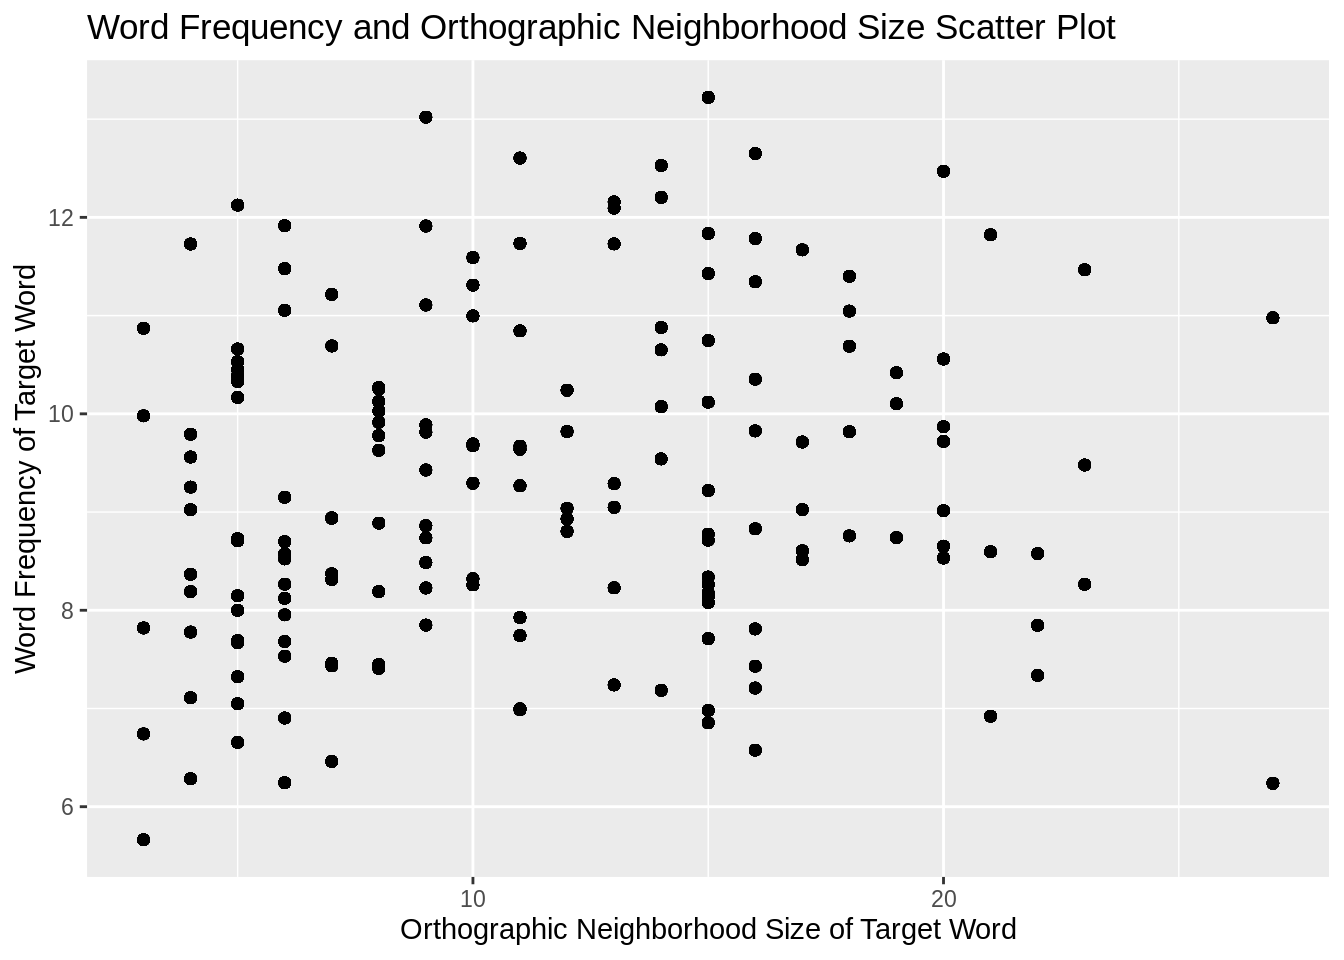
\includegraphics{bookdown-demo_files/figure-latex/unnamed-chunk-19-1.pdf}

\begin{longtable}[]{@{}cc@{}}
\toprule
Grammar Component & Specification\tabularnewline
\midrule
\endhead
data & mydata\tabularnewline
aesthetic mapping & x: OrthoN\_T, y: Freq\_T\tabularnewline
geometric object & points\tabularnewline
scale & x: linear, y: linear\tabularnewline
statistical transform & none\tabularnewline
coordinate system & rectangular\tabularnewline
facetting & none\tabularnewline
\bottomrule
\end{longtable}

\subsection{Example: Histogram Grammar}\label{example-histogram-grammar}

Useful for depicting the distribution of a continuous random variable.
Partitions the number line into bins of certain width, counts the number
of observations falling into each bin, and erects a bar of that height
for each bin.

Required aesthetics:

\begin{itemize}
\item
  \texttt{x}: A numeric vector.
\item
  By default, a histogram plots the count on the y-axis. If you want to
  use proportion (i.e., ``density''), specify the y = ..density..
  aesthetic.
\item
  You can change the smoothness of the plot via two arguments (your
  choice):
\item
  \texttt{bins}: the number of bins/bars shown in the plot.
\item
  \texttt{binwidth}: the with of the bins shown on the plot.
\end{itemize}

Let us say that we want to ask very, very specific questions about how
some word properties relate to other word properties. For example, in
this experiment we change one letter for a given letter position. for
example (word-work) pair manipulates the 4th letter position while
(worm-dorm) pair manipulates the 1rst letter position. Let us explore if
the words in a particular letter position category vary in word
frequency. The way we can do this is by using the \texttt{facet\_grid()}
function in \texttt{ggplot}.

\begin{Shaded}
\begin{Highlighting}[]
\NormalTok{mydata }\OperatorTok\StringTok{ }\KeywordTok{ggplot}\NormalTok{(}\KeywordTok{aes}\NormalTok{(}\DataTypeTok{x =}\NormalTok{ Freq_T)) }\OperatorTok{+}\StringTok{ }
\StringTok{  }\KeywordTok{geom_histogram}\NormalTok{(}\DataTypeTok{bins =} \DecValTok{20}\NormalTok{, }\DataTypeTok{alpha =}\NormalTok{ .}\DecValTok{7}\NormalTok{) }\OperatorTok{+}\StringTok{ }
\StringTok{  }\KeywordTok{xlab}\NormalTok{(}\StringTok{"Word Frequency of Target Word"}\NormalTok{) }\OperatorTok{+}\StringTok{ }
\StringTok{  }\KeywordTok{ylab}\NormalTok{(}\StringTok{"Count"}\NormalTok{) }\OperatorTok{+}\StringTok{ }
\StringTok{  }\KeywordTok{ggtitle}\NormalTok{(}\StringTok{"Word Frequency Distribution for Target Words"}\NormalTok{) }\OperatorTok{+}\StringTok{ }
\StringTok{  }\KeywordTok{facet_grid}\NormalTok{(}\OperatorTok{~}\NormalTok{probe_position) }\OperatorTok{+}
\StringTok{  }\KeywordTok{theme_classic}\NormalTok{() }
\end{Highlighting}
\end{Shaded}

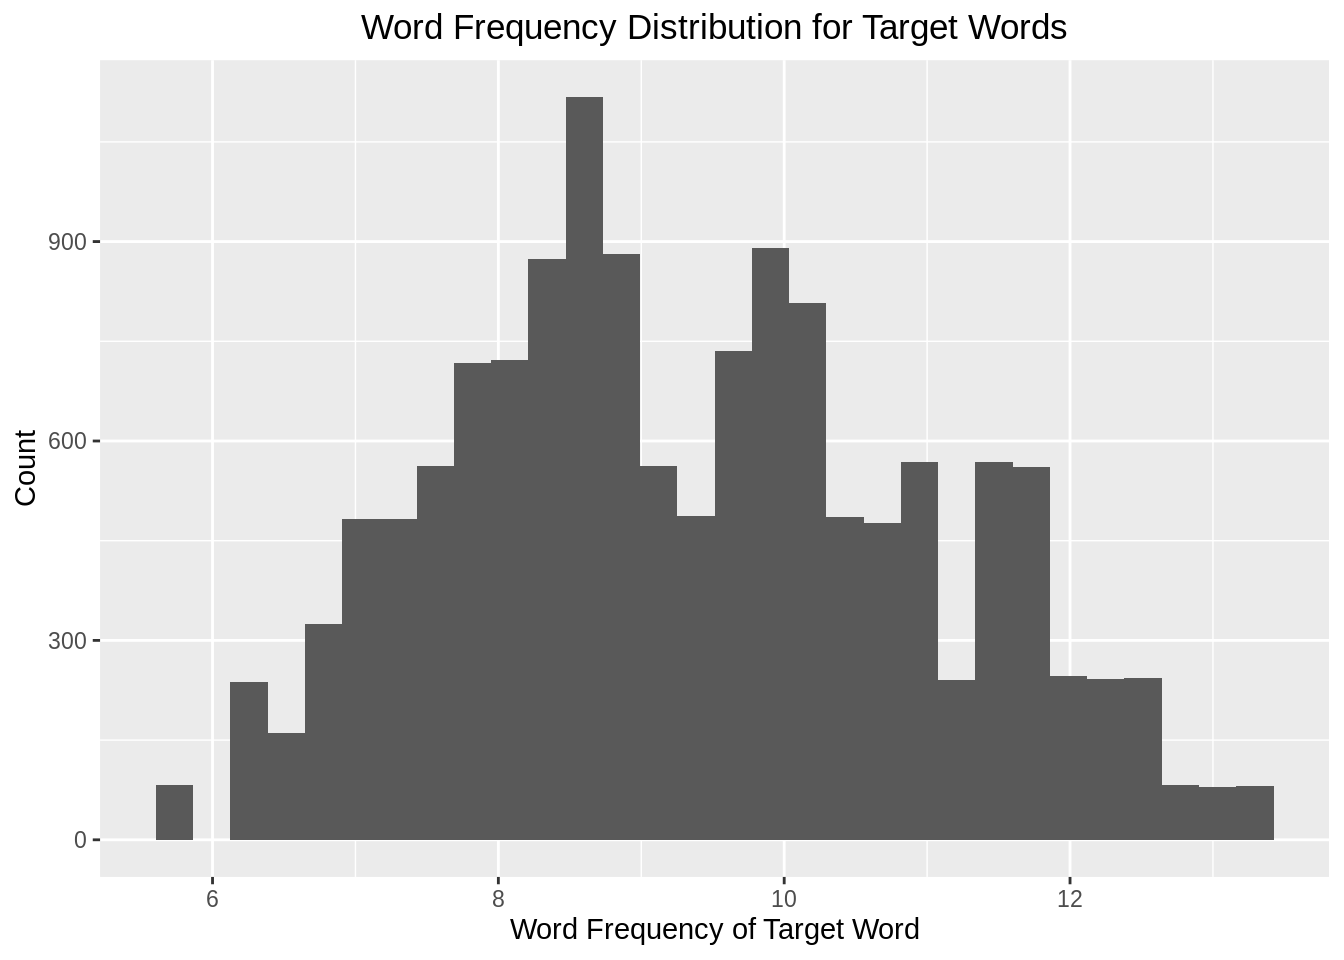
\includegraphics{bookdown-demo_files/figure-latex/unnamed-chunk-20-1.pdf}

\subsection{Example: Density Grammar}\label{example-density-grammar}

Essentially, a ``smooth'' version of a histogram. Uses kernels to
produce the curve.

Required aesthetics:

\begin{itemize}
\item
  \texttt{x}: A numeric vector. Good to know:
\item
  \texttt{bw} argument controls the smoothness: Smaller = rougher.
\end{itemize}

Let us say that we want to explore the same question from before, but we
felt like the last graphic wasn't as clear as we would want it to be. We
could use a different graphing strategy such as the density plot to make
it clearer to whoever is intepreting the data. Data is only as good as
you can communicate and understand it. Observe the differences between
the last code's output and this code's output

\begin{Shaded}
\begin{Highlighting}[]
\NormalTok{mydata }\OperatorTok\StringTok{ }\KeywordTok{ggplot}\NormalTok{(}\KeywordTok{aes}\NormalTok{(}\DataTypeTok{x =}\NormalTok{ Freq_T)) }\OperatorTok{+}\StringTok{ }
\StringTok{  }\KeywordTok{geom_density}\NormalTok{(}\KeywordTok{aes}\NormalTok{(}\DataTypeTok{fill =} \KeywordTok{factor}\NormalTok{(probe_position), }\DataTypeTok{alpha =} \FloatTok{0.05}\NormalTok{)) }\OperatorTok{+}\StringTok{ }
\StringTok{  }\KeywordTok{xlab}\NormalTok{(}\StringTok{"Word Frequency of Target Word"}\NormalTok{) }\OperatorTok{+}\StringTok{ }
\StringTok{  }\KeywordTok{ylab}\NormalTok{(}\StringTok{"Count"}\NormalTok{) }\OperatorTok{+}\StringTok{ }
\StringTok{  }\KeywordTok{ggtitle}\NormalTok{(}\StringTok{"Word Frequency Distribution for Target Words"}\NormalTok{) }\OperatorTok{+}\StringTok{ }
\StringTok{  }\KeywordTok{scale_fill_discrete}\NormalTok{(}\DataTypeTok{name =} \StringTok{"Probe Position"}\NormalTok{, }\DataTypeTok{labels =} \KeywordTok{c}\NormalTok{(}\StringTok{"1"}\NormalTok{, }\StringTok{"2"}\NormalTok{, }\StringTok{"3"}\NormalTok{, }\StringTok{"4"}\NormalTok{)) }\OperatorTok{+}
\StringTok{  }\KeywordTok{theme_classic}\NormalTok{() }
\end{Highlighting}
\end{Shaded}

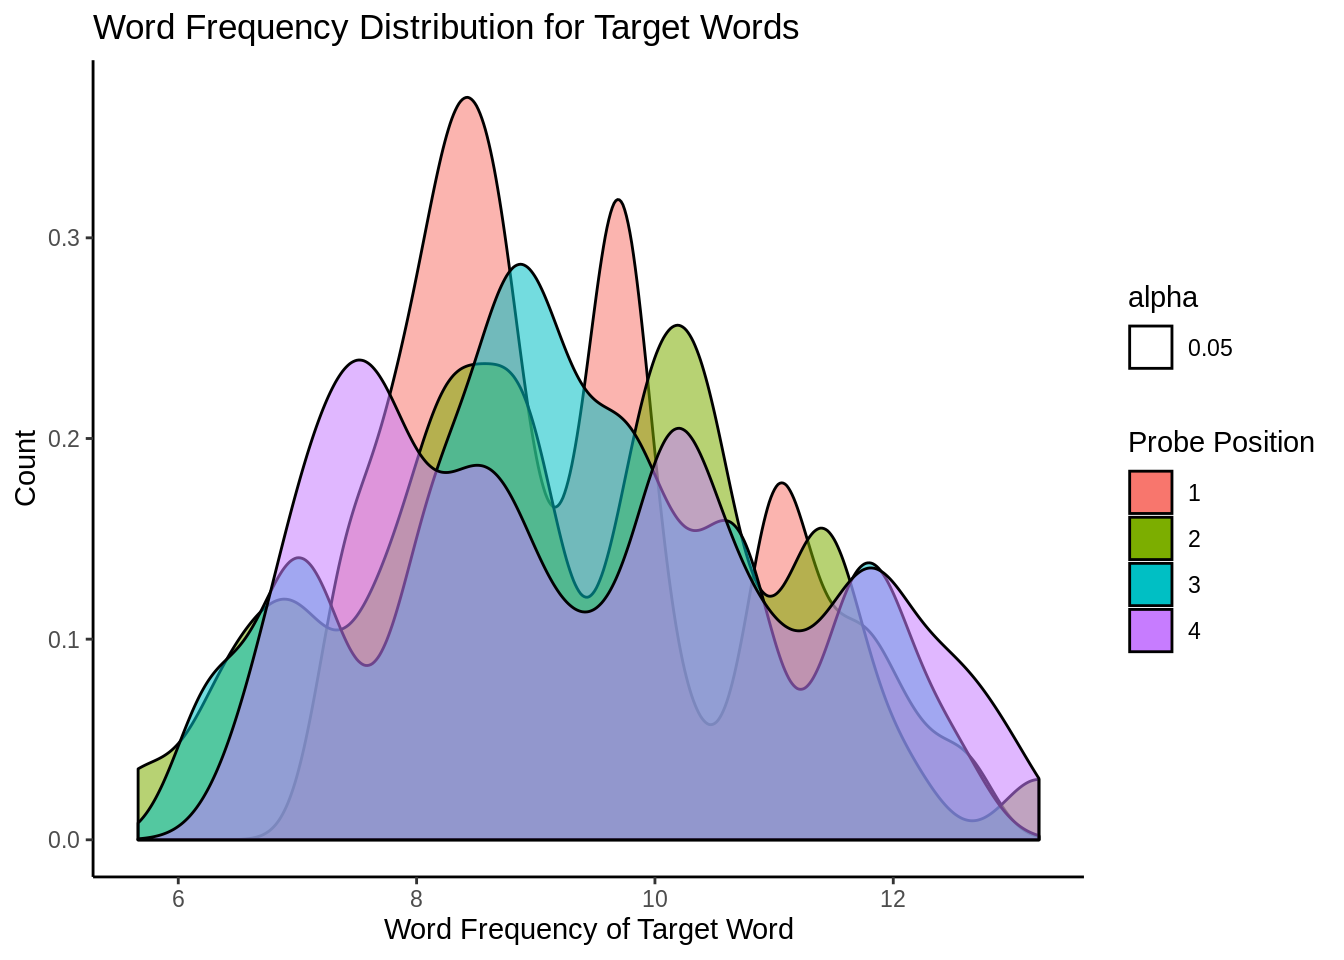
\includegraphics{bookdown-demo_files/figure-latex/unnamed-chunk-21-1.pdf}

\section{Plotting: Experimental
Analysis}\label{plotting-experimental-analysis}

In cognitive psychology we are particularly interested in how our
independent variables and participant variables influence performance on
a particular task. In this section we are going to plot performance on
this study's task. We are going to view a few ways to graphically
represent how these variables influence performance.

\subsection{Plotting Levels of One Categorical
Variable}\label{plotting-levels-of-one-categorical-variable}

One of our manipulations for this study was visual field. Staub and
Goddard (2019) argue that it is easier to identify words when they are
presented in foveal vision as compared to parafoveal vision. This is
ostensibly due to the fact that visual clarity drops as a function of
eccentricity (how many degrees from central vision is the target word).
To test this hypothesis, we will simply graph how people perform on a
task across visual field. Here is an example.

\begin{Shaded}
\begin{Highlighting}[]
\NormalTok{mydata }\OperatorTok\StringTok{ }\KeywordTok{ggplot}\NormalTok{(}\KeywordTok{aes}\NormalTok{(}\DataTypeTok{x =}\NormalTok{ visual_field, }\DataTypeTok{y =}\NormalTok{ accuracy)) }\OperatorTok{+}\StringTok{ }
\StringTok{  }\KeywordTok{geom_point}\NormalTok{(}\DataTypeTok{size =} \DecValTok{3}\NormalTok{) }\OperatorTok{+}\StringTok{ }
\StringTok{  }\KeywordTok{xlab}\NormalTok{(}\StringTok{"Visual Field"}\NormalTok{) }\OperatorTok{+}\StringTok{ }
\StringTok{  }\KeywordTok{ylab}\NormalTok{(}\StringTok{"Correct Responses"}\NormalTok{) }\OperatorTok{+}\StringTok{ }
\StringTok{  }\KeywordTok{ggtitle}\NormalTok{(}\StringTok{"Correct Responses as a Function of Visual Field"}\NormalTok{) }\OperatorTok{+}\StringTok{ }
\StringTok{  }\KeywordTok{theme_classic}\NormalTok{() }
\end{Highlighting}
\end{Shaded}

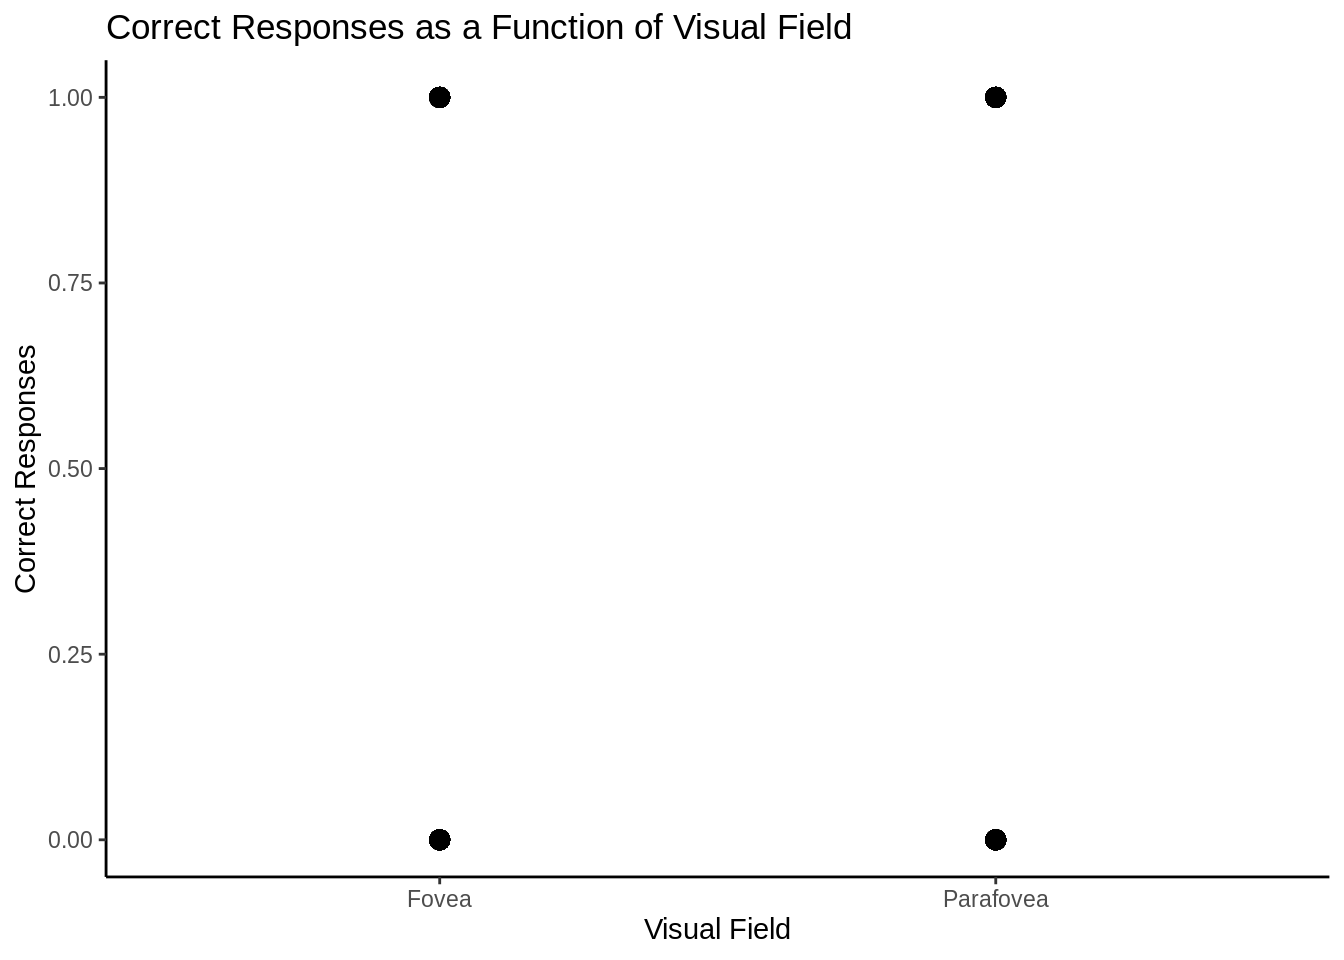
\includegraphics{bookdown-demo_files/figure-latex/unnamed-chunk-22-1.pdf}

\begin{Shaded}
\begin{Highlighting}[]
\CommentTok{# stat_summary(fun.data = "mean_se", geom = "pointrange")}
\end{Highlighting}
\end{Shaded}

Now you may see that there is something wrong with this graph. In fact,
there isn't, the problem is that all of the response data is binary:
coded as (0) when you are incorrect, and (1) when you are correct. Since
participants got right and wrong answers in both levels on the
condition, they look identical. Thus, a better way to plot this is to
create a summarized version of the data in each level of visual field.
Here is an example.

\begin{Shaded}
\begin{Highlighting}[]
\NormalTok{mydata }\OperatorTok\StringTok{ }\KeywordTok{ggplot}\NormalTok{(}\KeywordTok{aes}\NormalTok{(}\DataTypeTok{x =}\NormalTok{ visual_field, }\DataTypeTok{y =}\NormalTok{ accuracy)) }\OperatorTok{+}\StringTok{ }
\StringTok{  }\KeywordTok{stat_summary}\NormalTok{(}\DataTypeTok{fun.data =} \StringTok{"mean_se"}\NormalTok{, }\DataTypeTok{geom =} \StringTok{"pointrange"}\NormalTok{, }\DataTypeTok{size =}\NormalTok{ .}\DecValTok{8}\NormalTok{) }\OperatorTok{+}\StringTok{ }
\StringTok{  }\KeywordTok{xlab}\NormalTok{(}\StringTok{"Visual Field"}\NormalTok{) }\OperatorTok{+}\StringTok{ }
\StringTok{  }\KeywordTok{ylab}\NormalTok{(}\StringTok{"Correct Responses"}\NormalTok{) }\OperatorTok{+}\StringTok{ }
\StringTok{  }\KeywordTok{ggtitle}\NormalTok{(}\StringTok{"Correct Responses as a Function of Visual Field"}\NormalTok{) }\OperatorTok{+}\StringTok{ }
\StringTok{  }\KeywordTok{theme_classic}\NormalTok{() }
\end{Highlighting}
\end{Shaded}

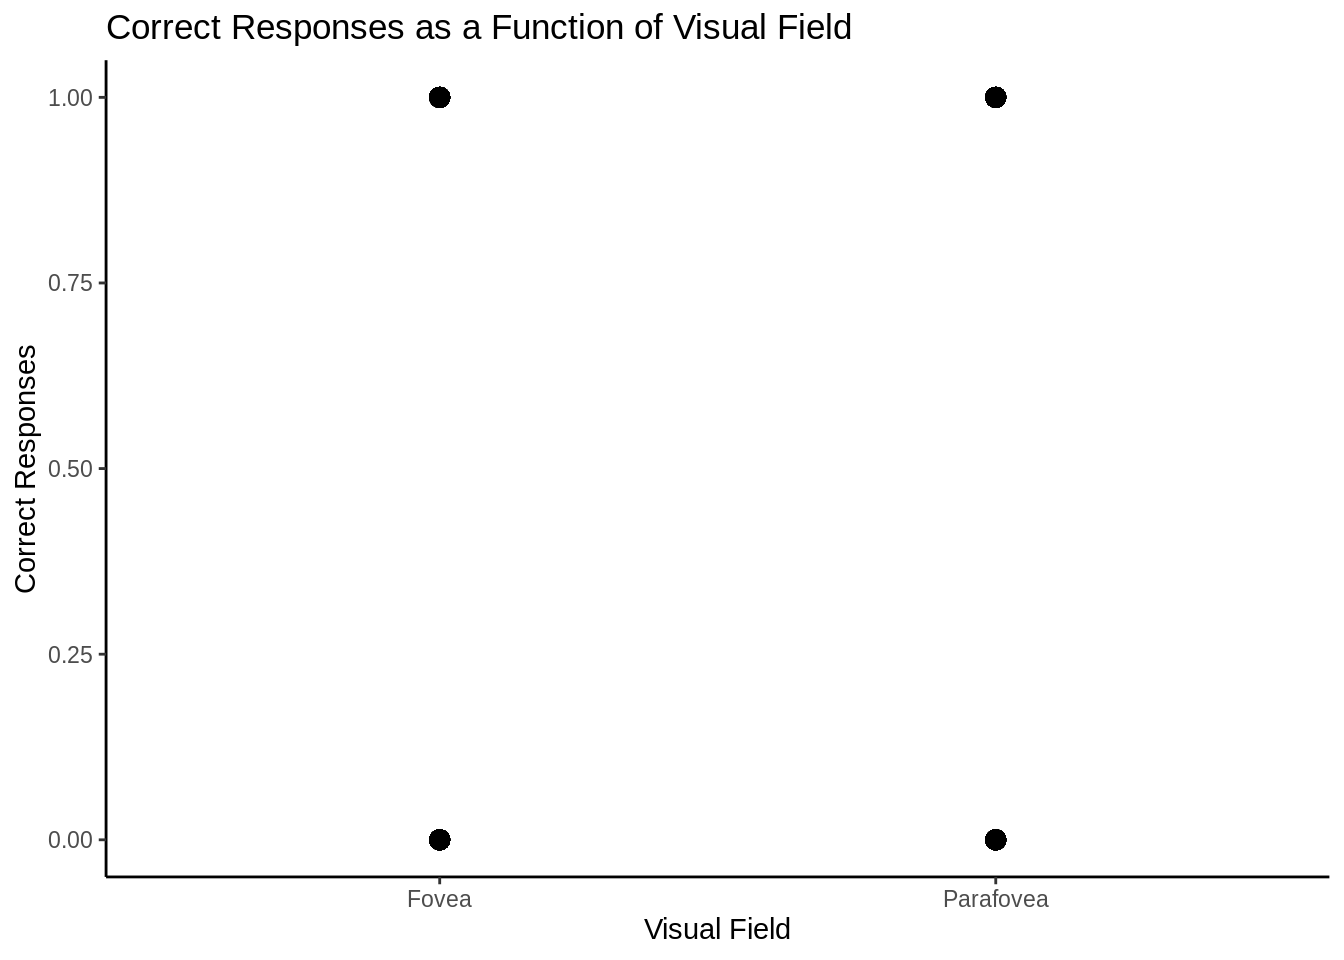
\includegraphics{bookdown-demo_files/figure-latex/unnamed-chunk-23-1.pdf}

\bibliography{book.bib,packages.bib}

\end{document}
